\documentclass[conference]{IEEEtran}
\IEEEoverridecommandlockouts
% The preceding line is only needed to identify funding in the first footnote. If that is unneeded, please comment it out.
\usepackage{cite}
\usepackage{amsmath,amssymb,amsfonts}
\usepackage{algorithmic}
\usepackage{graphicx}
\usepackage{textcomp}
\usepackage{xcolor}
\def\BibTeX{{\rm B\kern-.05em{\sc i\kern-.025em b}\kern-.08em
    T\kern-.1667em\lower.7ex\hbox{E}\kern-.125emX}}
\begin{document}

\title{Data Analysis\\
{\footnotesize \textsuperscript{*} This project is made for INF356}
}

\author{\IEEEauthorblockA{1\textsuperscript{st}Ömer Ertekin}
\IEEEauthorblockA{\textit{Computer Science} \\
\textit{Galatasaray University}\\
Istanbul, Turkey \\
omer.ertekin.gsu@gmail.com}

}

\maketitle



\section{Introduction}
In this document, we will describe and analyse our dataset for predicting the winner

\section{Purpose of this analysis}

It is very difficult to predict the course of the match in football. The match played between each team can progress differently from each other. You have to be very lucky to be able to predict match results without any data. What if we have data? Can we predict the winner by analyzing this data? At least can we make some guesses for the bet coupon?

\section{Main question and sub-questions}
In this section we will try to divide our problem to smaller parts and try to gather info for answering the main question.


\subsection{Main Question : Who will win?}\label{AA}
There are thousands of factors that will affect the match score.It's really hard to guess and that's why it makes the most money. For answering this question,
we will try to examine some of factors that will affect the winner of the match.

\subsection{Sub-questions}
\begin{itemize}
\item Which team is better ? : This question will have a great impact about score because as we said,every single match can progress differently. And that's 
the main reason for this difference.
\item Can both teams score? : This is a common type of bet and we will shape our score prediction based on the information from this question. There are hundreds of factors that will affect this situation. Therefore we need another questions.
\item How many shots did the teams take to score a goal? : Since we will examine how many positions the teams have entered and how many shots did the
teams took, we would have a statistics that will answer to this question.
\item How many cards did the teams get? :A yellow card can make a huge difference in the defensive performance of the teams in terms of hardness. A red card 
would make a bigger difference in game because the team is missing one or more person. Therefore, it will be very difficult for you to create the appropriate area in terms of offense and defense.
\item Who plays a more dominant game? :The more you dominant, the more chances you have to score, the less chance of conceding a goal. We have various data to understand who plays more dominant like possession percent, pass percent,aerials won count etc.
\end{itemize}

\section{Our Data}
We have 98 team from 5 major soccer league in the world and their data about different things. So let's take a look at data that we have and examine some of the analysis

\subsection{Goals}
We have data on the number of goals scored by teams over the entire season. This data will definitely help us in predicting the score of the match.As you can see from the figure 1, the number of goals has a normal distribution. Its mode (50) , median(50)  and mean (52.18)  are very close to each other.

\begin{figure}[h]
  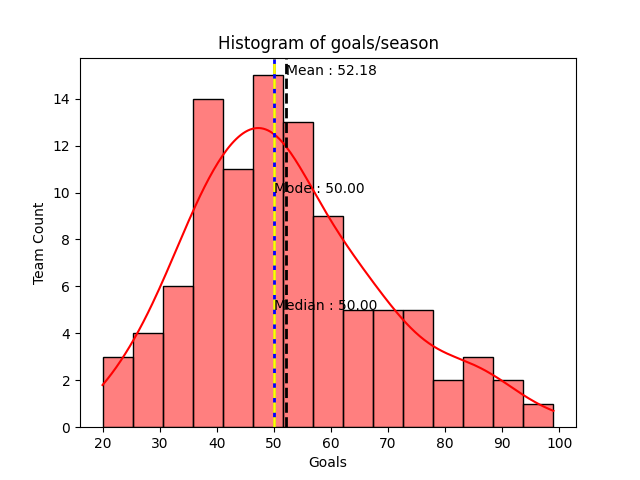
\includegraphics[width=\linewidth]{GoalFigure.png}
  \caption{Goals per season.}
  \label{fig:boat1}
\end{figure}



\subsection{Shots Per Game}
You can't score without shoting ( at least most of time ). Therefore, we will examine this data together with the goal scored data to measure the team's goal scoring ability. As you can see in figure 2, its mode (11.60) , median(11.45)  and mean (11.85)  are not very far to each other so we could say that it has a normal distrubition.

\begin{figure}[h]
  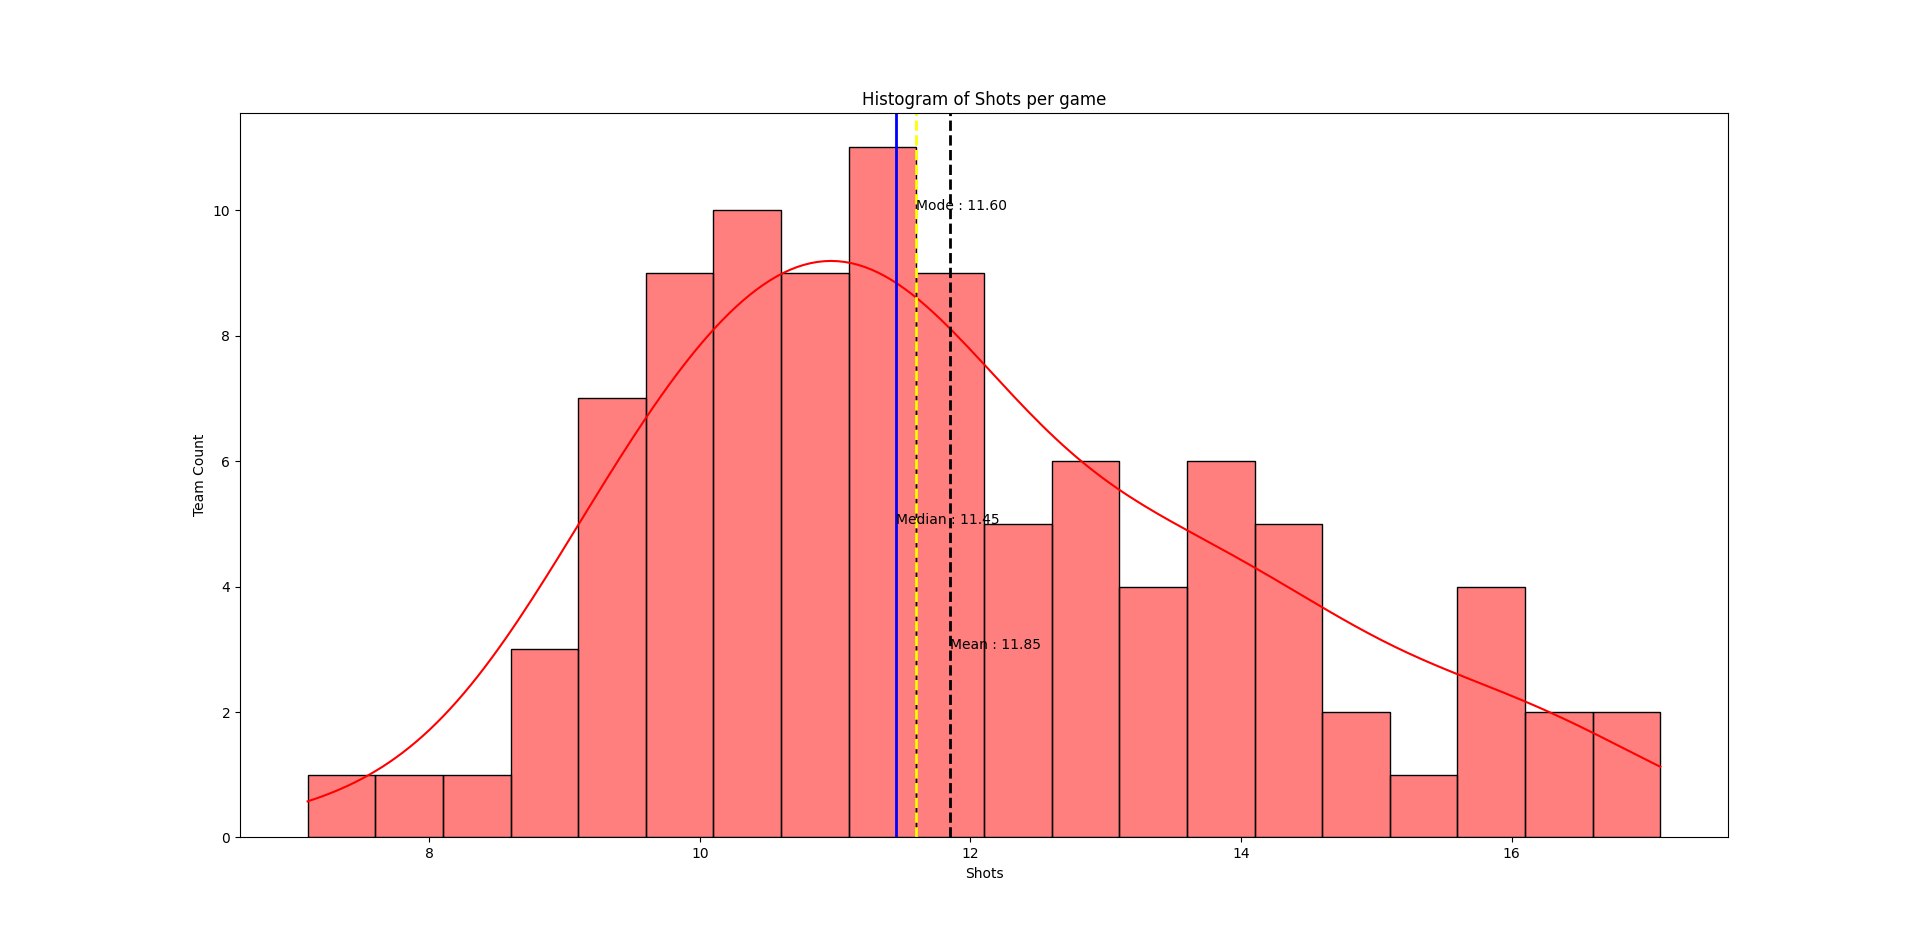
\includegraphics[width=\linewidth]{ShootsPg.png}
  \caption{Shots Per Game.}
  \label{fig:shotspg}
\end{figure}


\subsection{Cards}
Cards will affect the attack and defense performance. And each type/number of card will have a different effect. That's why we will examine each card separately
\subsubsection{Yellow Cards}
If a player is shown the yellow card, he/she has to be much more gentle when making his/her next defensive action. That's why it will affect the match score.
Like other data, we can say that yellow cards has a normal distrubition too with mode = 63, median 67.5, mean 69.70 in Figure 3.

\subsubsection{Red Cards}
Red cart directly effect the game because the more players you have on the field, the easier it is to find a position and the harder the opponent finds a position.  In figure 4, With mean = 3.34, mode = 3, median = 3, data has a normal distrubition 


\begin{figure}[h]
  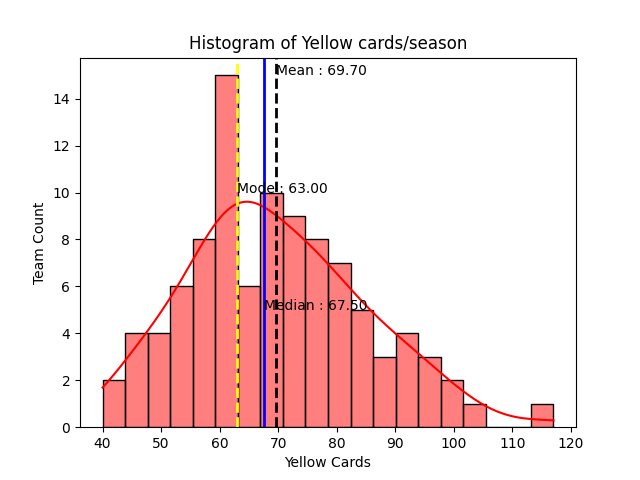
\includegraphics[width=\linewidth]{YellowCardFigure.png}
  \caption{Yellow card per season.}
  \label{fig:yc}
\end{figure}


\begin{figure}[h]
  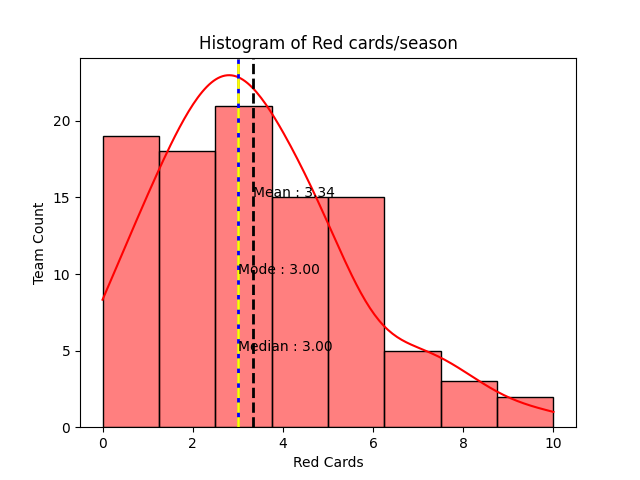
\includegraphics[width=\linewidth]{RedCardFigure.png}
  \caption{Red card per season.}
  \label{fig:yc}
\end{figure}

\subsection{In-game advantages}
You can dominate your opponent in different ways in the game. Some teams dominate the game by winning too many airballs or the team doesn't lose the ball because most of its passes are accurate. Or, since the percentage of possession is very high throughout the match, the team finds easier positions and does not give the ball to the opponent. For that we need to analyse this 3 type of data and combine them.
\subsubsection{Possession\%}
This data does not give very precise information about the score of the match. Because it is possible for teams to have a high percentage of ball possession and not be able to score. However, it can still provide information about the progress of the match. As we can see in Figure 5, posession\% has a distrubition like normal. Its mean = 50, median = 49.75 and mode = 51.5
\subsubsection{Pass\%}
Like Possession, this data isn't very precise too. But it will effect the match so we will examine it in Figure 6. Mode = 82.53, Median = 80.80 and Mean = 80.44. A normal distrubition.
\subsubsection{Aerials Won}
That data will effect the defence and attack performance. Let's have a look at Figure 7. Mode  = 18.30, median = 16.10, mean = 16.01. So close! That's why it has a normal distrubition

\begin{figure}[h]
  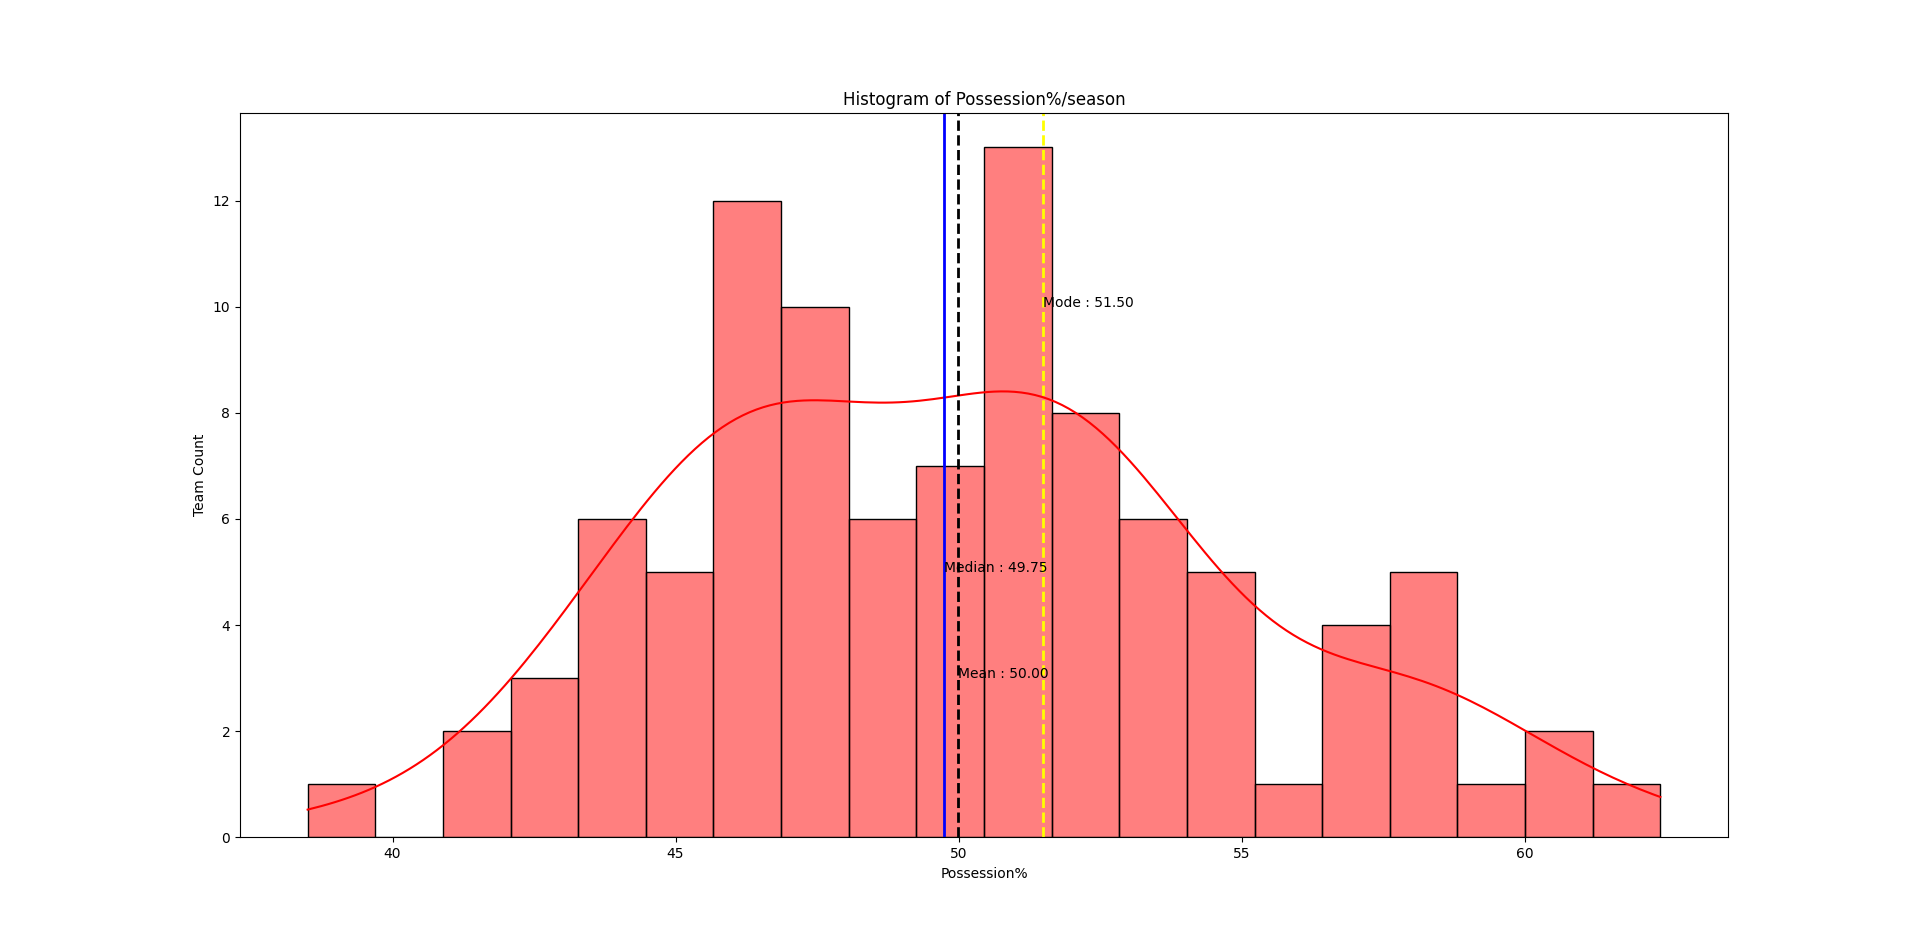
\includegraphics[width=\linewidth]{Possession.png}
  \caption{Average possession\%/season.}
  \label{fig:possession}
\end{figure}

\begin{figure}[h]
  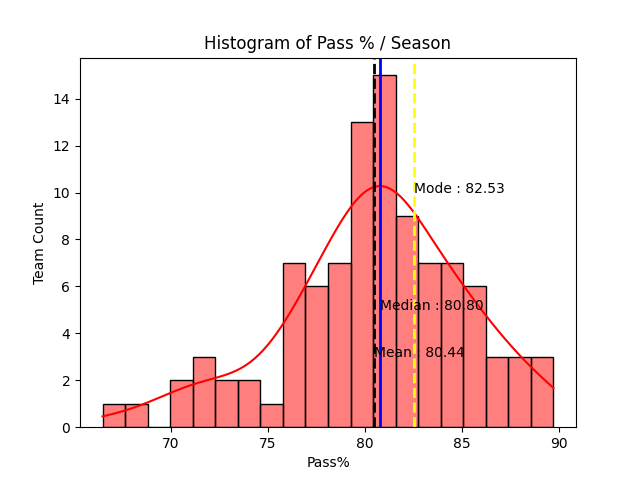
\includegraphics[width=\linewidth]{Pass.png}
  \caption{Average pass accuracy\%/season.}
  \label{fig:pass}
\end{figure}

\begin{figure}[h]
  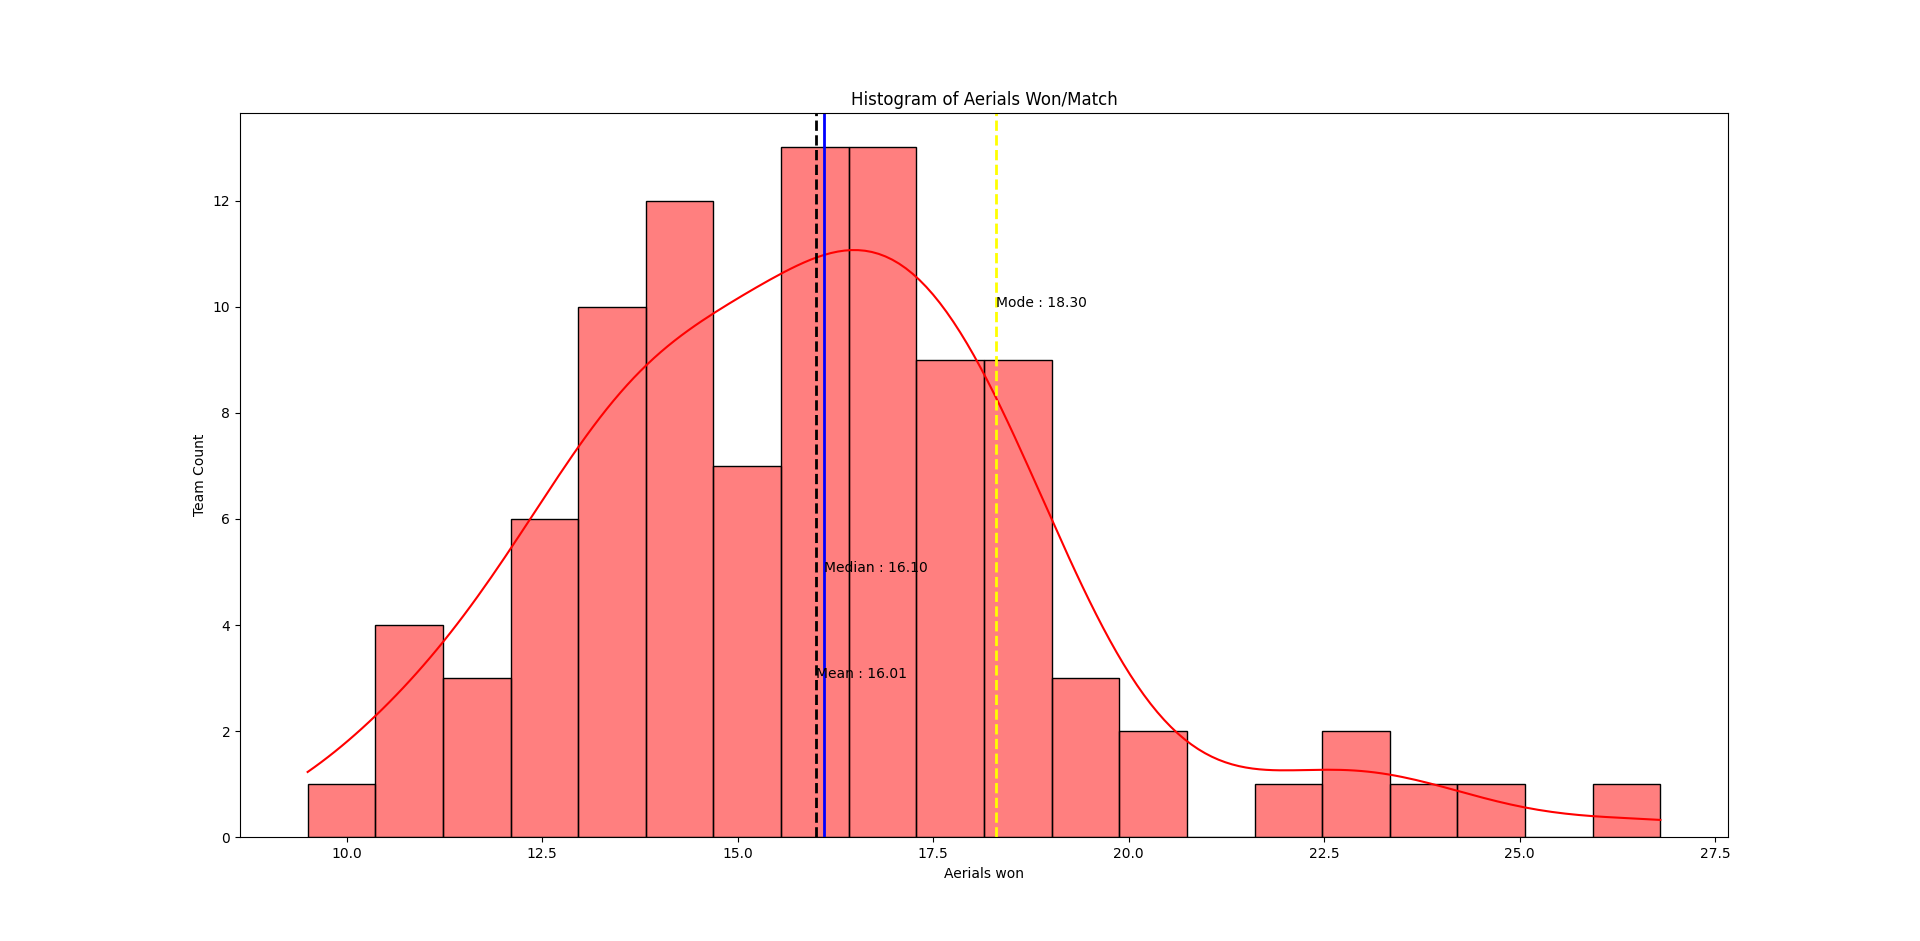
\includegraphics[width=\linewidth]{AerialsWon.png}
  \caption{Aerials won/per match.}
  \label{fig:aerial}
\end{figure}

\subsection{Team ratings}
When two teams meet each other, it will be difficult to score goals according to the level of the teams. Therefore, analyzes made independently of this data will not yield logical results. Let's look at this analysis at Figure 8. It has bimodal distrubition with Mode = 6.63, median = 6.65, mean = 6.55

\begin{figure}[h]
  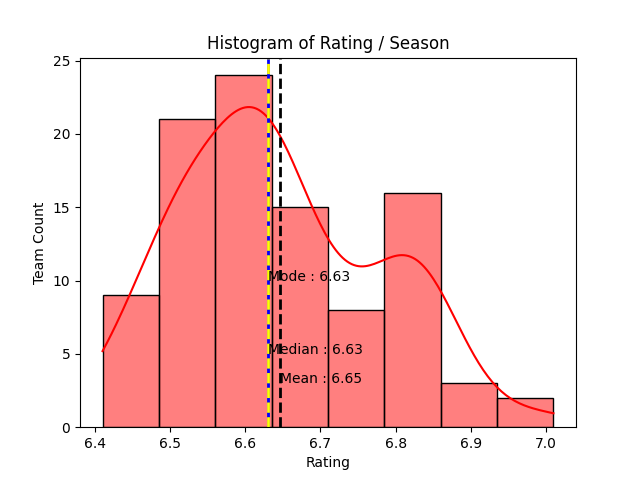
\includegraphics[width=\linewidth]{Rating.png}
  \caption{Ratings in season.}
  \label{fig:rate}
\end{figure}


\section{Examine our data to use}
Since we have enough data to use, let's try to examine which of these data are related to each other. Than we will use related data
and try to predict the winner of matches.
\subsection{Overview to variables}
The most important thing to predict the winner is goal count. If we could predict the team which will score more, we would find the winner of the match. In that case we can start by examining the variables that can affect the number of goals and the relationship between these variables. But before, let's look at all of the correlations between variables at figure 9.
\begin{figure}[h]
  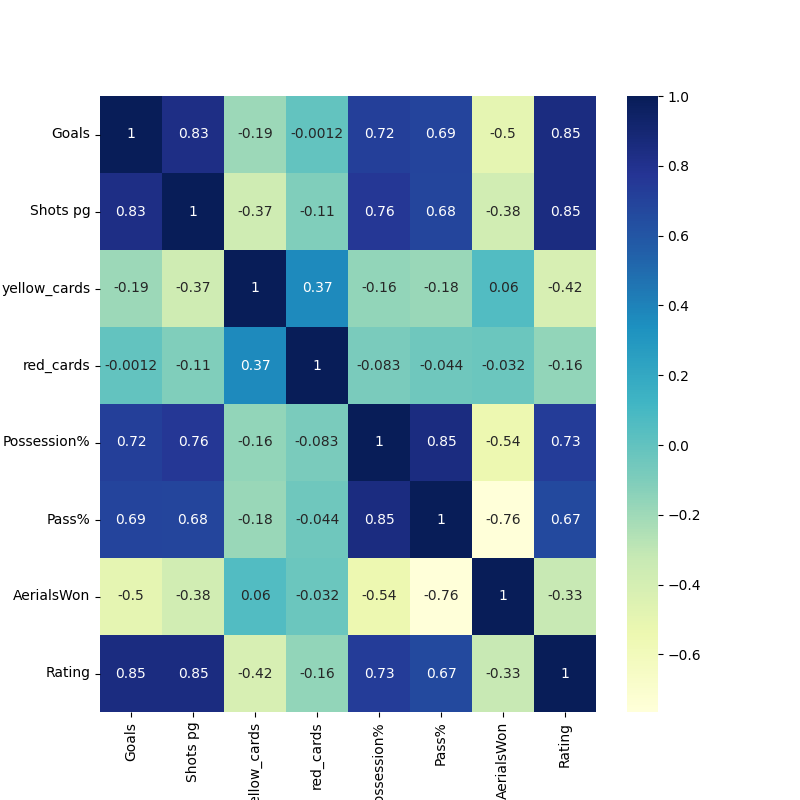
\includegraphics[width=\linewidth]{HeatMap.png}
  \caption{Correlation matrix heatmap.}
  \label{fig:heat}
\end{figure}


\subsection{Look at data pairs}
We will take some pairs to examine and try to catch a correlation between these two datas. And we will use these pairs to predict our score in our final analysis
 
\subsubsection{Goals and Shots Per Game}
The duo, which we expect to be the most relevant to each other at first glance, does not mislead us when we look at its graph.We can clearly see that there is a positive correlation between shots and goals in Figure 10. Our correlation coefficient is 0.83 which is really close to 1

\begin{figure}[h]
  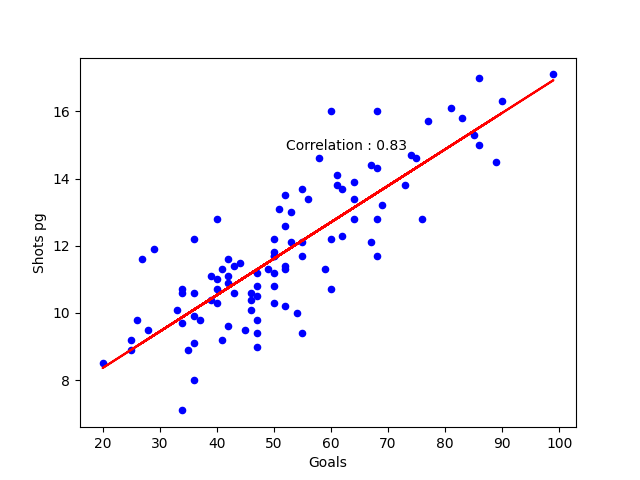
\includegraphics[width=\linewidth]{Shots_Goal_corr.png}
  \caption{Goals and shots correlation.}
  \label{fig:Shots_Goal_corr}
\end{figure}

\subsubsection{Goals and Team Ratings}
The more you score, the better team you are. And the data is confirming us. We can directly say that goal counts and team ratings are relevant(positively). As we can see in figure 11 ,correlation coefficient is 0.85.

\begin{figure}[h]
  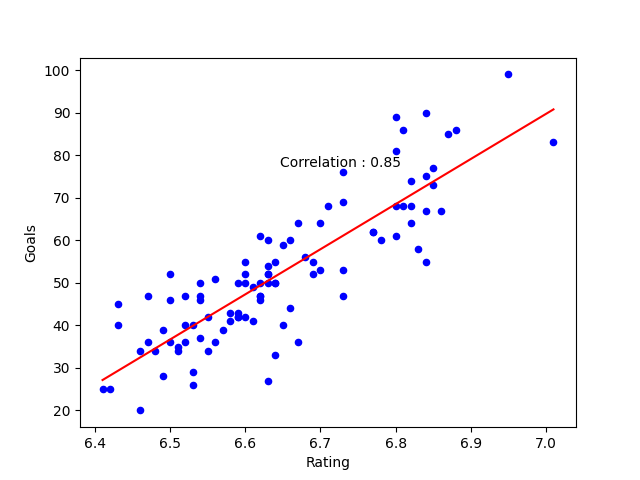
\includegraphics[width=\linewidth]{Goal_rank_corr.png}
  \caption{Goals and rank correlation.}
  \label{fig:Goal_rank_corrr}
\end{figure}


\subsubsection{Pass and Possessions}
The more accurate your passes, the longer the ball stays on your feet. Therefore, it is inevitable that these two are related to each other. The pass will affect the team overal power and we will use it to predict our winner. Let's look at positive correlation between pass and possesions in figure 12


\begin{figure}[h]
  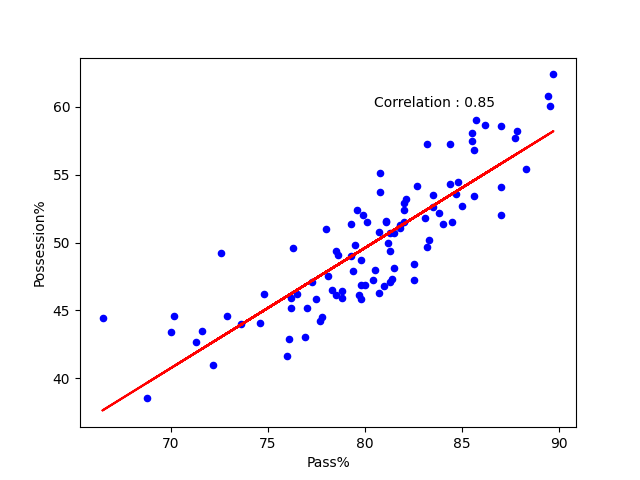
\includegraphics[width=\linewidth]{Pass_possesion_corr.png}
  \caption{Pass and possession correlation.}
  \label{fig:Pass_possesion_corr}
\end{figure}

\subsubsection{Yellow cards and Red cards}
Two yellow cards mean one red cards. So they must be relevant isn't it? No. It is strange but no they haven't a clear correlation. We can examine their relation in figure 13

\begin{figure}[h]
  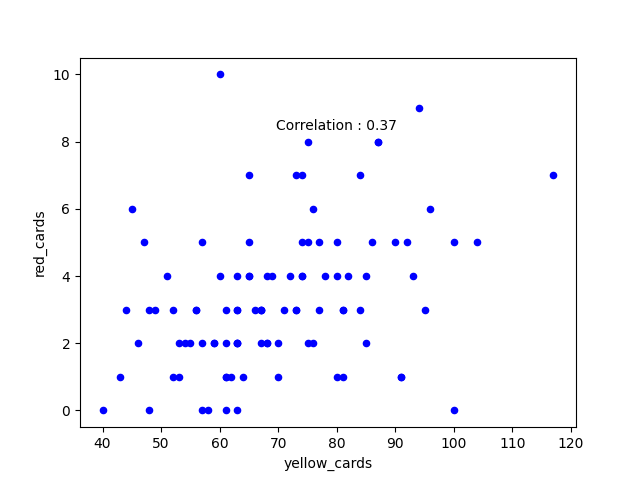
\includegraphics[width=\linewidth]{yellow_red_corr.png}
  \caption{Yellow and Red Cards correlation.}
  \label{fig:yellow_red}
\end{figure}

\subsubsection{Possesion and Aerials Won}
This pair may seem a little unrelated. But actually they aren't completely inrelevant. Teams with a higher percentage of ballplay this season have won less airballs. We can see negative correlation between these two data in figure 14

\begin{figure}[h]
  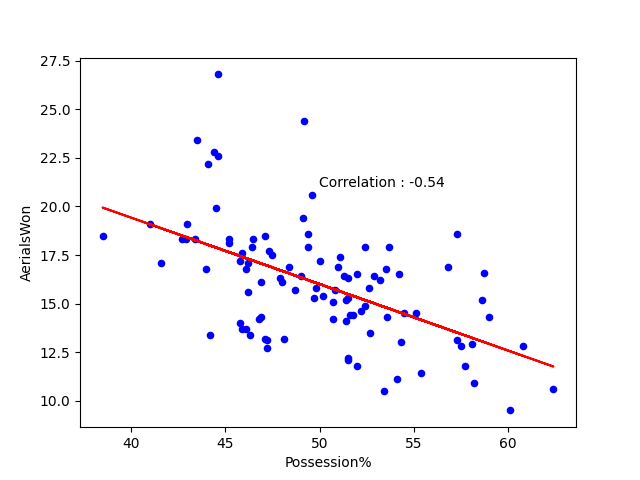
\includegraphics[width=\linewidth]{poss_aerials_corr.png}
  \caption{Possession and Aerials won correlation.}
  \label{fig:poss_aerials_corr}
\end{figure}

\subsubsection{Possession and Rating}
Even some teams have a different strategy like counter attack, in general good teams play more with ball. Our data is confirming us as we can see in figure 15. There is a positive correlation.

\begin{figure}[h]
  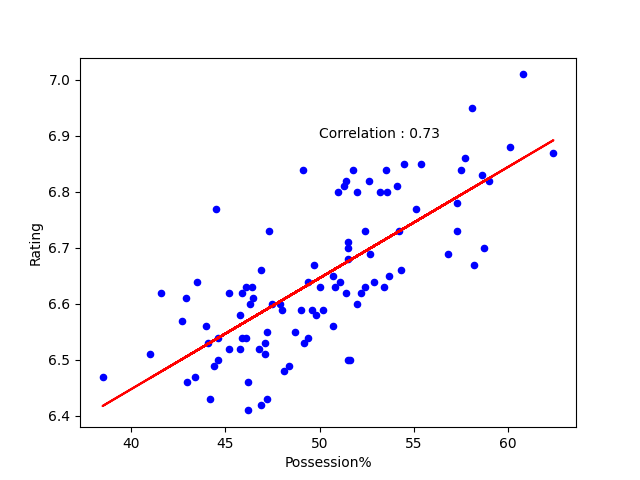
\includegraphics[width=\linewidth]{pos_rating_corr.png}
  \caption{Possession and Rating correlation.}
  \label{fig:pos_rating_corr}
\end{figure}


\subsection{Look at all of pairs}

We selected some pairs from our data and examined the relationship between them. We will use interrelated data to complete our analysis. We will try to determine the outcome of the possible match of the teams using each of its associated data. At figure 16, there is a complete pair plot of our data to see clearly the relations between data frames.

\begin{figure}[h]
  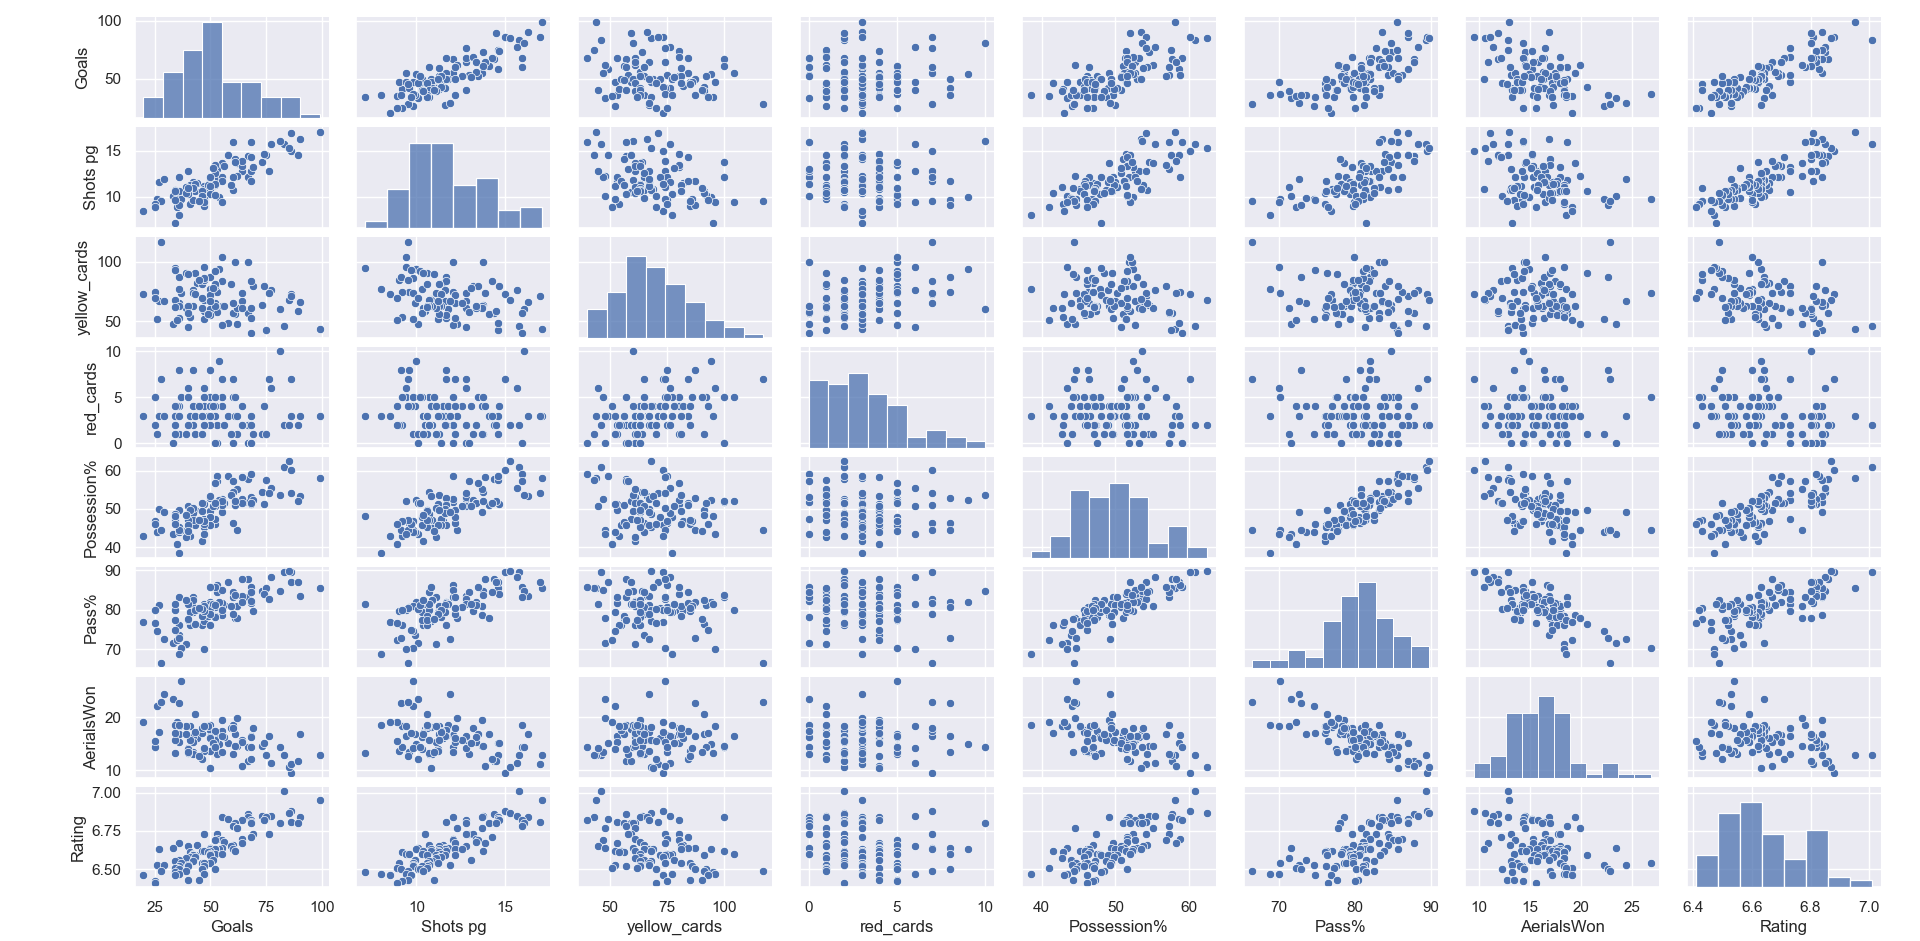
\includegraphics[width=\linewidth]{PairPlot.png}
  \caption{All data pairs.}
  \label{fig:pairplot}
\end{figure}


\end{document}
